\chapter{Robustness Analysis}
\label{Chapter-Robustness-Analysis}

Maybe this need its own chapter\\
Developed FL architecture. Server - Client architecture, communication protocol, tf embeddment. Interface - code agnostic of NN design and training.

The experiments from the reviews. Add a prologue to show why they exist. Remake the supplementary ones with the latest settings.

%%%%%%%%%%%%%%%%%%%%%%%%%%%%%%%%%%%%%%%%%%%%%%%%%%%%% Software %%%%%%%%%%%%%%%%%%%%%%%%%%%%%%%%%%%%%%%%%%%%%%%%%%%%% 
\section{Software}
\subsection{Tensorflow \& Keras}
TensorFlow \cite{tensorflow2015-whitepaper} is an interface for expressing ML algorithms and an implementation for executing such algorithms. It offers a complete, flexible ecosystem of tools, libraries and community resources that that facilitates the development and deployment of ML powered applications. Its main advantage is the ability to use high-level APIs like Keras with eager execution, enabling immediate model iteration and easy debugging. 

Tesnorflow \& Keras were used in all experiments during modelization. It is chosen due to its simple, flexible architecture, which turns new ideas into code quickly. In addition, due to the existence of TensorFlow Federated (TFF) \cite{tff} framework, there are many compatible theoretical resources and tutorials. TFF is simulating FL to facilitate research and experimentation with FL algorithms, thus it is incompatible with this work which aims to implement real-world FL with hardware accelerators.

\subsection{Python/C API} \label{Python/C API}
As the goal is to integrate FL with FPGA accelerators, the majority of the codebase is developed in C++. This include all the networking, communication, model aggregation and any required model transformations. TensorFlow on Python is utilized for model evaluation and, throughout the modelization phase, for training. To connect these two components, the Python interpreter is embedded to the core program using the Python/C API \cite{Python/C_API, embedding_python}.

With the TensorFlow C API \cite{TF_C_API}, TensorFlow could be used directly in C++, however several capabilities, like the Neural Network library, are not supported. Furthermore, quickly rotating among ANN architectures, training techniques, etc. is quite usual in FL development. With the C API that becomes tedious and slow, since it is geared more toward uniformity and simplicity than convenience, and C++ needs to be recompiled after every change. Due to these factors, integrating the Python interpreter and using TensorFlow in Python is considered as a more appropriate solution.

\subsection{POSIX sockets}
POSIX sockets \cite{POSIX_socket} is an application programming interface (API) for Internet and Unix domain sockets, used for inter-process communication (IPC). A socket is an abstract representation for the local endpoint of a network communication path. According to the Unix philosophy, the POSIX sockets API defines it as a file descriptor that offers a standard interface for input and output to data streams.

The 4.2 Berkeley Software Distribution \cite{bsd} Unix operating system, which was introduced in 1983, is where the API originates from. POSIX sockets transitioned mostly unchanged from a de facto standard to a POSIX specification component. They are commonly referred to as "Berkeley sockets" or "BSD sockets" to acknowledge the Berkeley Software Distribution, where they were first implemented.
 
In FL, entities possess their own private data. This is best implemented through processes with private data space that communicate using sockets. Therefore, the POSIX socket API implementation provided by the LINUX operating system is used for all inter-entity communication. 

POSIX sockets can be configured for blocking or non-blocking operation. In blocking operation, the program halts until the entire message is sent or received. In contrast, during non-blocking operation they only retrieve or send data that is immediately available. Thus, the program does not stall on straggler connections and many deadlock situations are avoided, but there is no guarantees that the messages will be send or received in one piece, especially when said messages are large \footnote{This is due to limited sized socket buffers set up by the operating systems.}.

%%%%%%%%%%%%%%%%%%%%%%%%%%%%%%%%%%%%%%%%%%%%%%%%%%%%% Data Preparation %%%%%%%%%%%%%%%%%%%%%%%%%%%%%%%%%%%%%%%%%%%%%%%%%%%%% 
\section{Data Preparation}
\subsection{Normalization}
Dataset normalization \cite{dataset_norm}, as part of data preparation, is a standard practice in ML. Normalization transforms the features of a dataset to a common scale, without distorting discrepancies in the ranges of values or losing information. This technique prevents large scaled characteristics to dominate during training. Furthermore, many algorithms, such as ReLU non-linearities, exhibit better performance when fed with data of floating-point format.

In this work, the Fashion-MNIST dataset provided by TensorFlow Datasets \cite{TFDS} collection is utilized. It is consisted of gray-scale images, where each pixel is represented by an integer in the range \([0,255]\). They are normalized to floating-point format in the range \([0,1]\) with the script \texttt{prepare\_dataset.py}. Furthermore, to avoid repeating this procedure for every experiment, the processed dataset is saved on disk.

\subsection{Distribution}
In FL, each client is meant to have their own unique, individualized dataset. Given that the provided Fashion-MNIST dataset is a single, concentrated collection, it must be distributed among the clients in order for federated training to be possible. Two approaches of partitioning the data among the clients are explored:

\subsubsection{IID}
The data are randomly partitioned in equally sized shards, one for every client. For example, if there are 10 clients, each will receive a shard containing 6000 examples. Although this distribution is not IID in the strictest sense\footnote{Due the shards being mutually exclusive, knowing that an example belongs to one of them indicates that it does not exist in others shards. Thus, knowledge about the other local datasets can be inferred and independence is violated.}, it is closer to a real-world scenario and many issues, such as class underrepresentation, can be easily avoided.

\subsubsection{non-IID}
Although statistical challenges are not the focus of this study, some testing with non-IID data has been done for sake of completeness. The dataset is broken up into shards, each of which includes examples from only one label. Each client receives two shards of different labels. If there are 10 clients, for instance, twenty shards will be produced, and each client will receive 3000 examples from two labels for a total of 6000 examples. Despite such a pathological non-IID distribution being atypical of a real-world scenario, it will assist investigate how severely the algorithms fail on extremely non-IID data.

\subsection{Pipeline}
The input pipeline that feeds the training data to the models is constructed using the \texttt{tf.data} API provided by TensorFlow. More specifically, before training begins, each client optimizes the use of its dataset by transforming it through caching, shuffling, batching, prefetching, and repeating. Additionally, this process is parameterized for flexibility and enable experimentation with different local dataset and batch sizes.

%%%%%%%%%%%%%%%%%%%%%%%%%%%%%%%%%%%%%%%%%%%%%%%%%%%%% Embedding Python Interpreter %%%%%%%%%%%%%%%%%%%%%%%%%%%%%%%%%%%%%%%%%%%%%%%%%%%%%
\section{Embedding the Python Interpreter}
As mentioned in section \ref{Python/C API}, the Python Interpreter is embedded on top of the C++ codebase. To make this integration as seamless as possible from both sides, an integration layer that operates as a wrapper for the C/Python API, has been developed. The C++ codebase can call Python code with simple function calls, while the Python code can access data from the C++ space like it would access data from its own space.

To achieve this, A number of steps need to be completed. First of all, a strait-forward abstract class is defined, which specifies a train and an evaluate function, as well as an input and an output model. The C++ codebase is interfacing with an implementation of this class. Its tasks include initializing the Python interpreter, loading the appropriate Python module, passing the necessary data and creating C++ function wrappers for the Python function.

Moving data from one side to the other can be trickier than it first appears. Using the appropriate API calls, such as \texttt{PyModule\_AddIntConstant}, simple constants and macros can be passed by copy to the Python module in a strait-forward manner. This approach fails when dealing with large amounts of data, such as the model parameters. Instead, by constructing NumPy array metadata over them and copying them, they can be passed by reference. In this manner, both ends observe the same memory space and there is no significant data copy.

After exposing the parameters to the Python code, one more step is necessary to enable the TesnorFlow library to be able to use them. In order to assign the received parameters to the model under training, they must be first transformed into TesnorFlow tensors with dimensions and shapes that match its layers. Likewise, to extract parameters from a model and expose them to the C++ codebase, its layers must be concated in a NumPy array.


\begin{figure}[H]
    \centering
        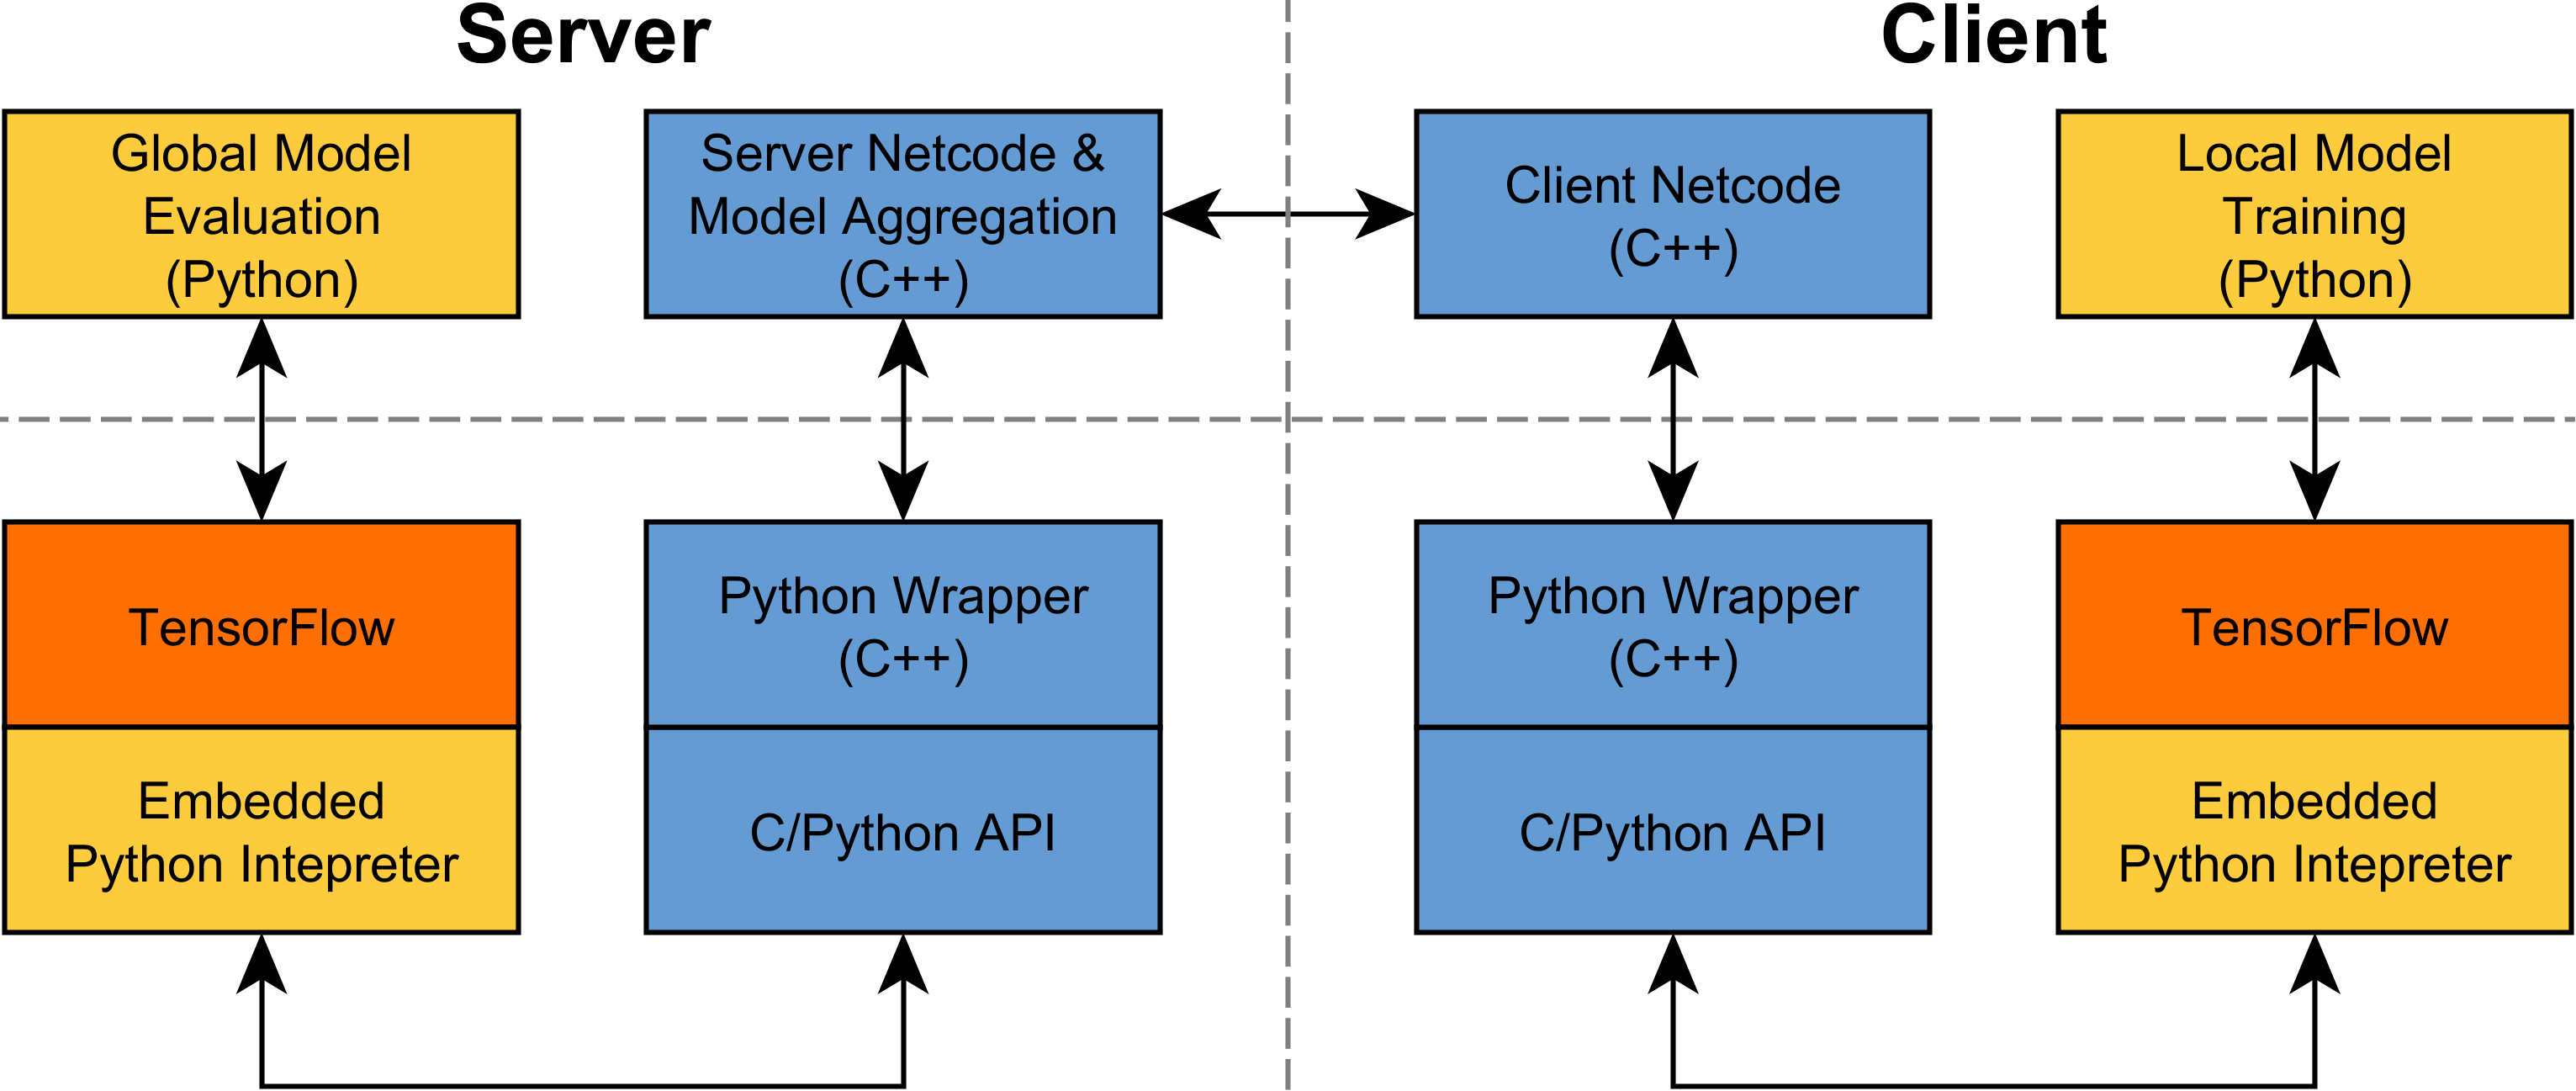
\includegraphics[width=1\textwidth]{Images/block_diagrams/model_lifecycle.png}
        \decoRule
        \caption[C++/Python Integration]{Overview of the C++/Python Integration. The FL protocol implementation components are represented by the top half, while the libraries, APIs, and wrappers needed to connect them are shown in the bottom half.}
        \label{fig:model_lifecycle}
\end{figure}

%%%%%%%%%%%%%%%%%%%%%%%%%%%%%%%%%%%%%%%%%%%%%%%%%%%%% implementation %%%%%%%%%%%%%%%%%%%%%%%%%%%%%%%%%%%%%%%%%%%%%%%%%%%%% 
\section{FL Architecture}
The architecture aims to offer a generalized FL loop that enables the implementation of various FL algorithms. To achieve this, it is designed to be flexible and modular, with each FL operation, such as client selection and aggregation, having its own specialized function. Additionally, all relevant training parameters and hyper-parameters, such as local epochs or participating clients per epoch, are compiled in the \texttt{definitions.hpp} file. Since the entire codebase accesses them from there, testing and experimentation are streamlined and less prone to mistakes.

In FL, multiple entities are present, the orchestrating server and the clients training the global model. As the aim of this work is to implement FL with clients operating on separate devices, it is essential that each entity is a distinct process with its own private data-space. That data-space contains its private training or testing dataset, as well as its local or global models. All required communication is facilitated through POSIX sockets.

\begin{figure}[H]
    \centering
        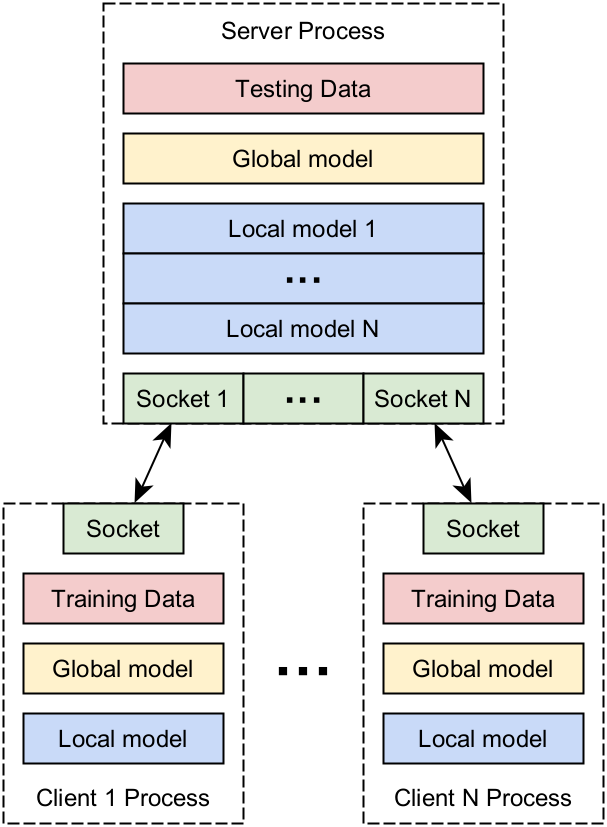
\includegraphics[width=0.5\textwidth]{Images/block_diagrams/memory_layout.png}
        \decoRule
        \caption[Process \& Memory layout]{Process and memory layout of the FL architecture. Each client holds their private data, the global model and the models they produced. Meanwhile, the server holds the testing dataset, the global model and the most recent local model it received. All communication goes through dedicated sockets.}
        \label{fig:process_mem_layout}
\end{figure}

\subsection{Server}
\subsubsection{Overview}
The server generally adheres to the event-driven server paradigm. The process, while sleeping, listens for events such as new connections or messages from the clients, and reacts according to their context. This is very similar to FL in that the server receives local models, aggregates them, and then, after accumulating a sufficient number of them, creates a new global model and announces it to the clients. All these actions are triggered by client updates.

The server process is the focal point of FL and is responsible for several tasks, which can be distinguished between algorithmic, systemic and auxiliary. Algorithmic tasks are the components of the FL algorithm, such as model aggregation. Systemic tasks are necessary operations to implement the FL algorithm, such as connecting sockets. In addition, some tasks that are not required to implement the algorithm are included in order to enhance its utility and ease development.

\subsubsection{Operation}
The server's first action is to load a pre-trained model, if one exists. While not a prerequisite to facilitate FL, this is done to enable transfer learning and experimenting with retraining a model under different settings. 

After that, the server completes a series of initializations. First of all, a listening socket is set-up in non-blocking operation, and the event-driven structure is established. Furthermore, the Python environment, where the global models are evaluated, is embedded and initialized. Finally, any structures or variables required by the FL algorithm are initialized.

After the initializations, the server enters a waiting state. To achieve this the \texttt{poll(2)} system call, which puts the process to sleep until an event occurs, is used. Four types of events may happen:
\begin{itemize}[leftmargin=*]
    \item The listening socket encounters a new connection, meaning a new client requests to join in the federated training. The socket is cloned, the clone establish the connection with the client, and any necessary data structures are created.
    \item A connected socket encounters an error, such as an sudden disconnection. Unreliable clients are expected to continue being unreliable, thus the most prudent course of action is discarding them.
    \item A connected socket receives new data. As a message can consist of millions of weights, it may be received across multiple events and a collection mechanism is needed to fully retrieve it. To achieve this, it is necessary to track the size of the received data per client and ensure that there is always adequate memory available to store a message from each connected client. If the message is complete and valid, its local model is aggregated to next global model, and the related client is considered as non-working.
    \item A connected socket can send new data. This indicates that a socket designated to send the global model to its connected client, is available to do so. As mentioned before, the messages can be quite large, thus multiple events may be required to fully send them. To achieve this, tracking of the amount of transmitted data per connection is necessary. When a message is fully send, the related client is considered as working. Furthermore, as there no more data to send, the \texttt{POLLOUT} flag of the socket is disabled.
\end{itemize}

Following any event, the server determines whether a new epoch should begin. It takes in consideration how many local models were successfully received this epoch, how many clients are connected, and how many clients are still working. If the current epoch requires further work, the process returns to the waiting state and sleeps until a new event occurs.

If the contrary is true, the new global model is created by dividing the aggregated local models by the number of received local models during the current epoch. Then, this new model is evaluated, and shared with randomly selected clients. The only action needed to share the model with a client is enabling the \texttt{POLLOUT} flag of the corresponding socket; the event loop will handle sending the message.

The event loop's final step is to determine whether any further training is required. If the target accuracy is achieved or a predetermined number of global epochs have been completed, the server shows any relevant statistics, stores the final global model to disk, and shuts down.

% \subsubsection{Memory layout}

\subsection{Client}
\subsubsection{Overview}
During an epoch, a participating client receives a global model, goes through a few local training rounds, and then sends the updated local model back to the server. Training cannot begin until the global model is fully received. Furthermore, after sending the local model, nothing further needs to be done until a new global model is received.

As a result, the client is controlled by its communication with the server, and a master-slave relationship is formed between them. To effectively implement this, client-side communication is blocking, meaning a client can not take any action until it has fully received or send its messages.

\subsubsection{Operation}
At startup, the client creates a socket and connects to the server. Additionally, it embeds and initializes the Python environment that is used for training.  Following these initializations, the process moves into its main loop.

The main loop contains three major operation. First, it receives the global model shared by the server. Then, it is trained with the local private data, creating a new local model. Finally, any required transformations, such as quantization and compression, are applied to the new model, which is then send to the server. This process is repeated until the server informs that there will be no more training with that client.

% \subsubsection{Memory layout}
\begin{figure}
    \centering
        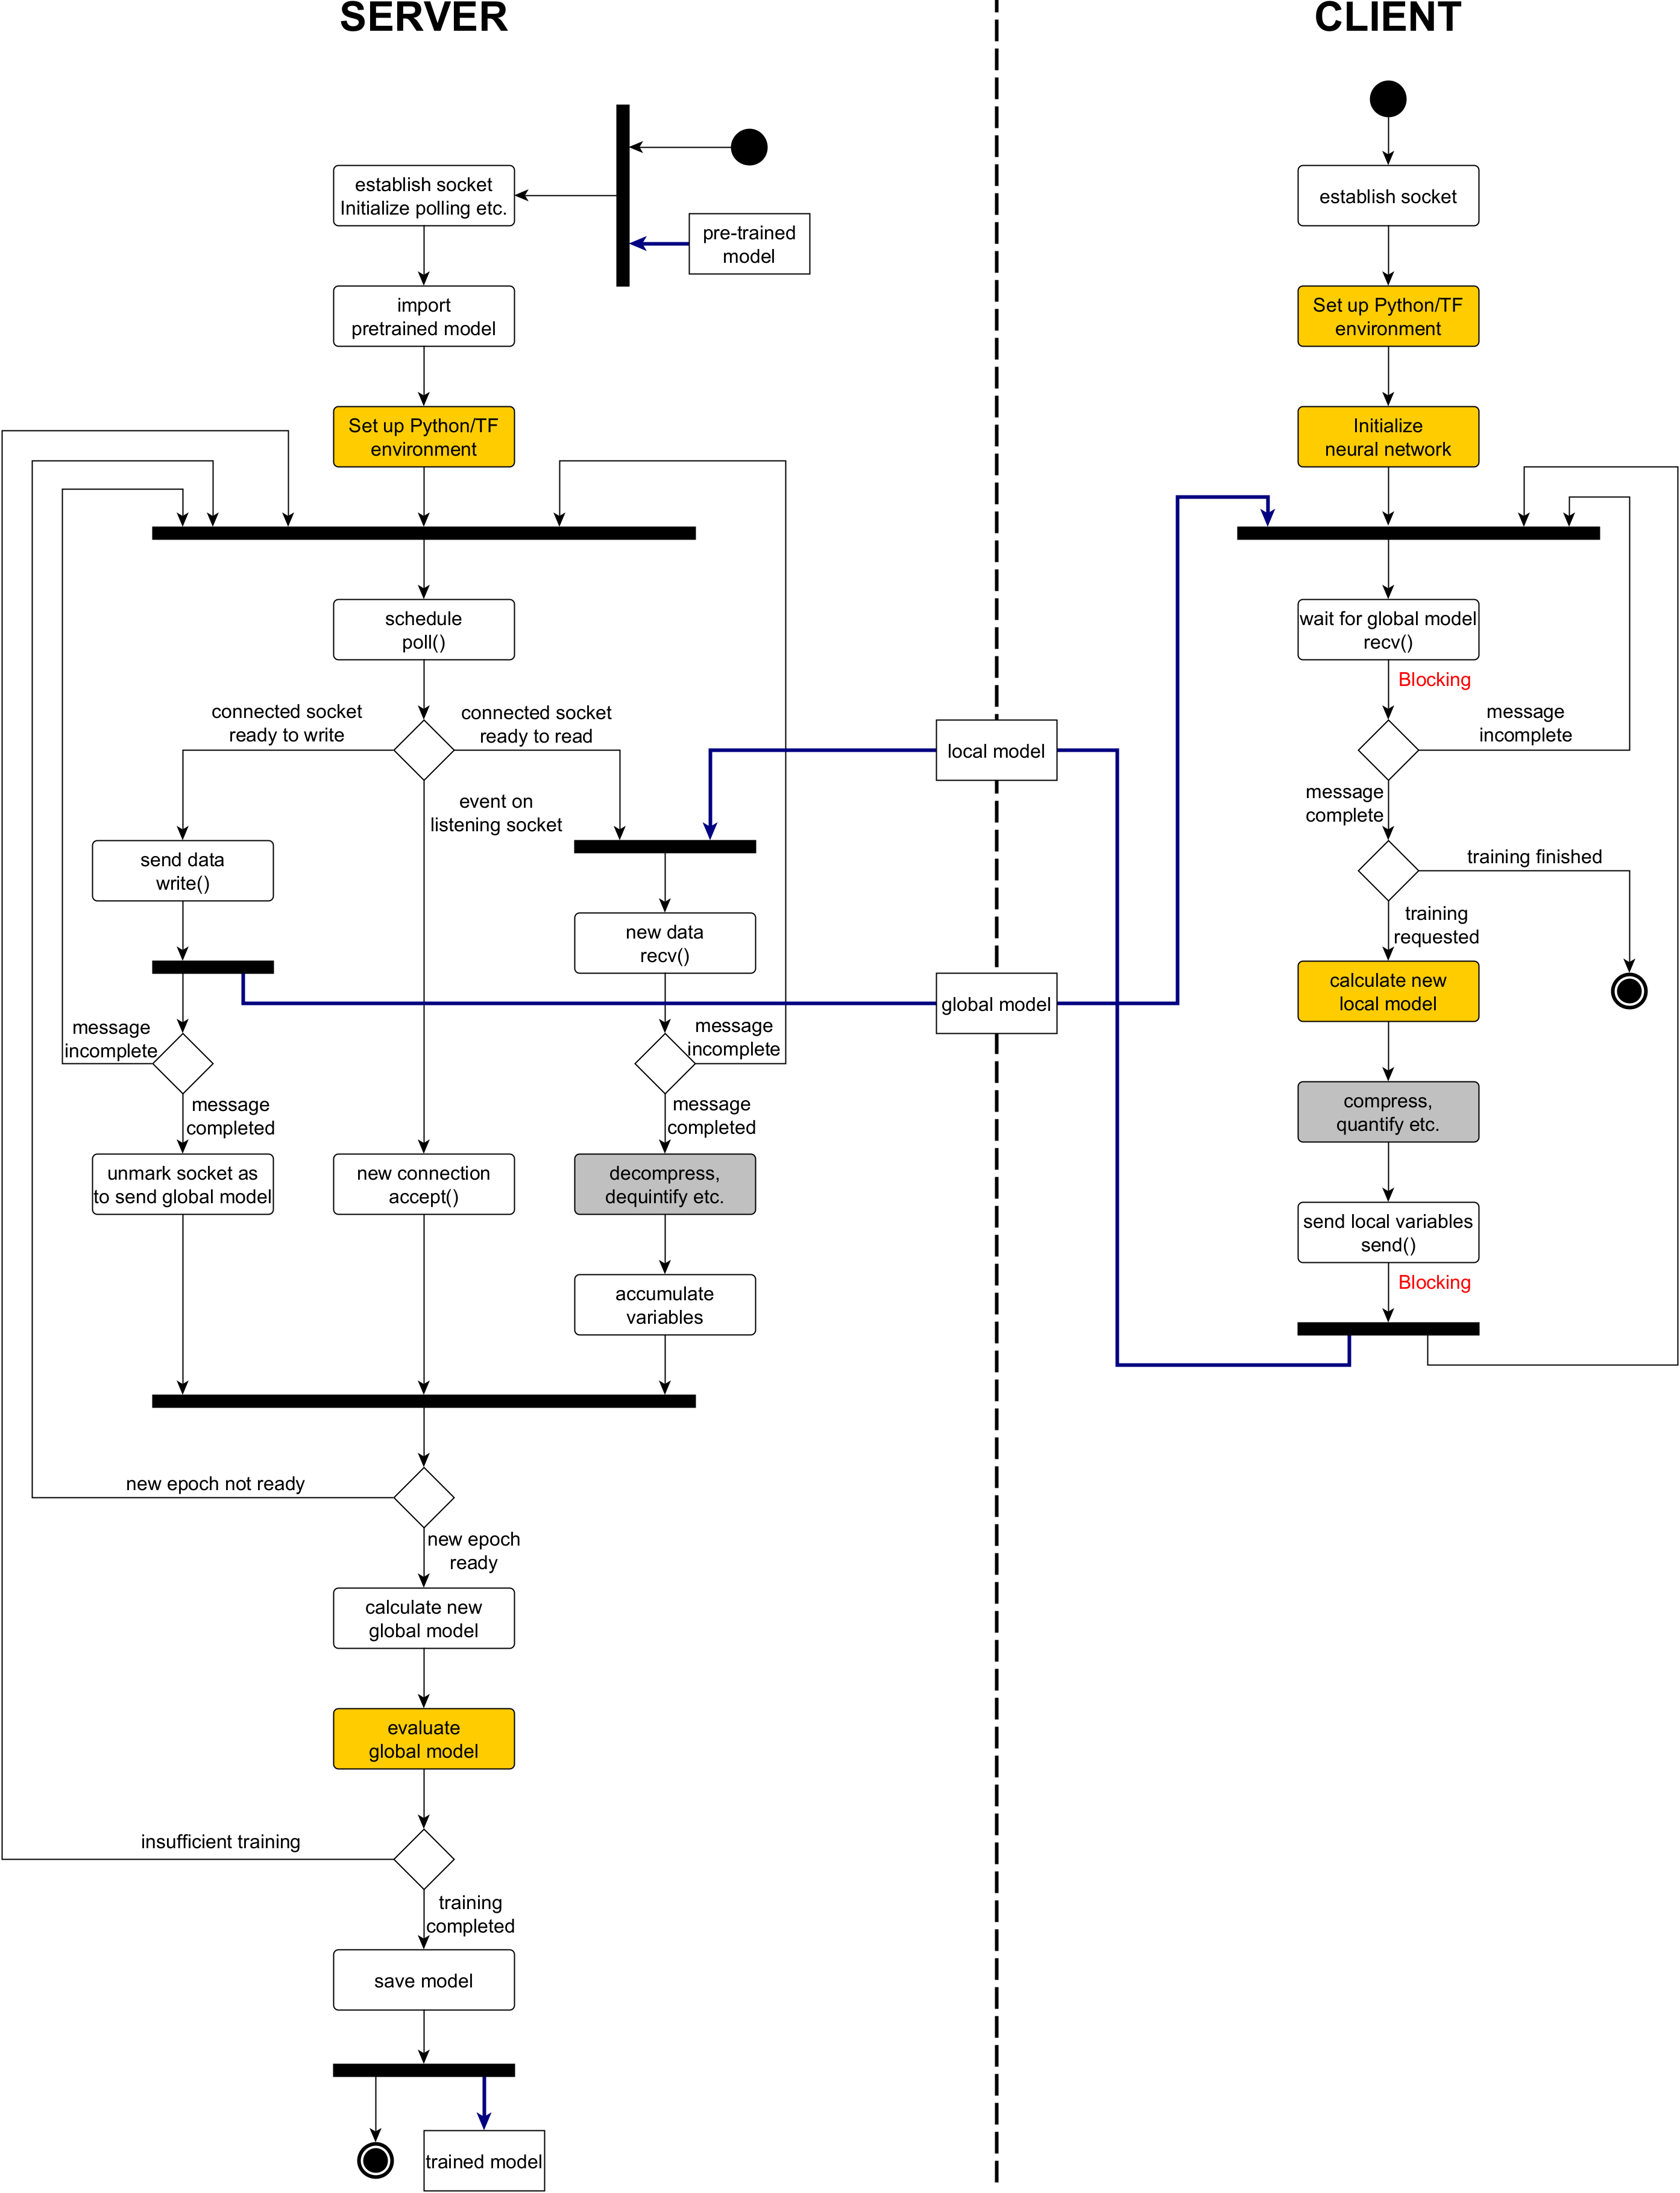
\includegraphics[ width=\textwidth, height=\textheight, keepaspectratio]{Images/block_diagrams/top.png}
        \decoRule
        \caption[Server - Client Activity Diagram]{Server - Client Activity Diagram: Yellow states are modelled with TensorFlow, while grey states are not essential for FL. Blue arrows represent data movements. Error conditions and states are not displayed.}
        \label{fig:server_client_activity_diagram}
\end{figure}
\subsection{Life cycle of a model?} figure 4.1

\subsection{Communication Scheme}
The FL training is set up to be cross-device compatible. The server holds minimum information about the clients, just enough to maintain connection and communicate. As a result, the server can not address clients directly and no confirmations are conveyed on any direction.

\subsection{Model Library}

% \section{Communication Scheme}
% The server and each client are separate processes with their own memory regions. Data must be shared efficiently and reliably, hence a fitting communication mechanism is required. This is accomplished by using messages with predetermined size and structure in order to reduce the frequency and complexity of the communication. The messages are C-aligned arrays and their structure is as follows.

% \begin{center}
%     \begin{tabular}{|c|}
%         \hline
%         Server to client message\\
%         \hline\hline
%         flags\\
%         \hline
%         global epoch\\
%         \hline
%         global model variables\\
%         ...\\
%         \hline
%         \multicolumn{1}{c}{ } \\
%     \end{tabular}
%     \quad
%     \begin{tabular}{|c|}
%         \hline
%         Client to server message\\
%         \hline\hline
%         global epoch\\
%         \hline
%         loss\\
%         \hline
%         accuracy\\
%         \hline
%         model variables / deltas\\
%         ...\\
%         \hline
%     \end{tabular}
% \end{center}

% The flags field is used to give orders or supplementary information to the clients. These are:
% \begin{itemize}
%     \item The received model is random and can be ignored.
%     \item The received model is the final one and no further communication will be accepted by the server.
% \end{itemize}
% The GE field is required for the server to determine whether a received model is addressed for the current GE and to accept or ignore it. The loss and accuracy fields can be used for more complex algorithms like disregarding local model with inadequate accuracy or greater loss than the previous GE.

% \medskip
% At the start of each GE, the server sends a message to each client chosen to take part, which is essentially an order to begin working. When a client finish its task, they answer with a single message containing the produced local network, indicating that they have completed their work. There is no need for any additional communication, such as confirmation or synchronization messages. In total 2 * N messages are sent every epoch, where N is the number of the clients. As far as the server is concerned, the clients are stateless and every interaction with them is unique. Each message is independent from the rest and must be self sufficient.



\section{Experiments}
point of experiments
what can we see, no timining look for global epochs
\subsection{Distributed SGD with IID data}
This experiment tests the algorithm with IDD distributed data. A simple CNN that classifies images of the Fashion MNIST dataset and the Adam optimizer are used. The neural network consists of approximately 420,000 Float32 trainable variables which produce messages of ~1.7MB. As the server and all the clients are running on the same machine, communication takes place on the operating system's loopback and no substantial timing can be made. The following experiment focus on model accuracy and the convergence rate of the FL algorithm in comparison to locally train a model. The training dataset, which consist of 60,000 images, is split equally between the clients. The following set of parameters and hyperparameters are set.

\begin{center}
    \begin{tabular}{|c|c|}
        \hline
        \multicolumn{2}{|c|}{ parameters } \\
        \hline\hline
        local epochs & 1 \\
        \hline
        steps per epoch & 3 \\
        \hline
        batch size & 10 \\
        \hline
    \end{tabular}
    \quad
    \begin{tabular}{|c|c|}
        \hline
        \multicolumn{2}{|c|}{ hyperparameters } \\
        \hline\hline
        global epochs & 500 \\
        \hline
        clients & 4 \\
        \hline
        \multicolumn{2}{c}{ } \\
    \end{tabular}
\end{center}

With these parameters and 4 clients per GE, all data will be passed once every 500 GEs. For the sake of clarity and to not be confused with the global and local epochs, each pass through all data is called a Session.

\medskip
The accuracy of the FL trained model is compared with the accuracy of a locally trained model. This model has the same batch size, and steps per epoch equal with the number of the data divided by the batch size. Thus, an epoch equals a Session. The following diagram shows the accuracy of the two models on the test data for each Session.

\begin{center}
    \begin{tikzpicture}
        \begin{axis}
            [
                xmin = 0,
                xmax = 21,
                xlabel = Session,
                xtick = { 1 , 2 ,..., 20 },
                ylabel = Test Accuracy,
                legend pos = south east,
                thick,
                scale = 1.25,
                every node/.style = {transform shape},
                scaled x ticks = false
            ]
            \addplot table [y=FL, x=P]{data/experiment1.dat};
            \addplot +[restrict x to domain=1:15] table [y=LL, x=P]{data/experiment1.dat};
            \addlegendentry{FL training}
            \addlegendentry{local training}
            
        \end{axis}
    \end{tikzpicture}
    \captionof*{figure}{Experiment 1 results}
\end{center}

\medskip
According to the diagram of the experiment, the FL trained model achieves the same accuracy as the locally trained model, albeit at a slower rate. The first model is updated every 150 examples while the second one every 10 examples. According to FL theory, the fewer are the examples that are used every GE, the faster the convergence is. Although, in that case more global epochs are required and the communication overhead increases. In contrast, if more examples are consumed each GE, less communication is required but the convergence rate is smaller and occasionally the model might not even converge. The original FL algorithm without deadline limitations achieved accuracy of 0.92 for Fashion-MNIST with IID data distribution which is comparable with the above results. Experiments with different parameters seems to corroborate this.

\medskip
Another observation from the above diagram is that FL training combats over-training in some degree. In the locally trained model, the training loss decreased with each step, however this did not translate to higher test accuracy. In contrast, the averaging of the FL algorithm can incur a rebalancing effect and pull out the local models from local extremum. During training the loss of the client models was not always decreasing.

\clearpage

\subsection{Distributed SGD with non-IID data}
In this experiment, the algorithm is tested with heavily unbalanced non-IID data and the previous neural network architecture. The fashion MNIST dataset is used and distributed between five clients. The first client holds all the examples with labels 0 or 1, the second client holds all the examples with labels 2 or 3 etc. This is an extreme case of unbalanced data, clients hold no knowledge of the other classes and if they train the network by themselves, a maximum accuracy of 20\% is achieved. In such cases, according to FL theory, better accuracy is achieved by minimizing the batch size and examples used per GE.

\medskip
For this experiment batch sizes of 1,2 and 4 are used. The local epoch and steps per epoch are set to 1. The global epochs are set in such a way that all data are passed once every session.

    \begin{center}
        \begin{tikzpicture}
            \begin{axis}
                [
                    xmin = 0,
                    xmax = 21,
                    xlabel = Session,
                    xtick = { 1 , 2 ,..., 20 },
                    ylabel = Test Accuracy,
                    legend pos = south east,
                    thick,
                       scale = 1.25,
                    every node/.style = {transform shape},
                    scaled x ticks = false
                ]
                \addplot table [ x=P , y=b1 ]{data/experiment2.dat};
                \addplot table [ x=P , y=b2 ]{data/experiment2.dat};
                \addplot table [ x=P , y=b4 ]{data/experiment2.dat};
                
                % \addplot [ very thin , blue ] 
                %     gnuplot [raw gnuplot] {
                %          f(x) = a * x^3 + b * x^2 + c * x + d;
                %          a = 0.0001;
                %          b = 0.0001;
                %          c = 0.1;
                %          d = 80;
                %          fit f(x) 'data/experiment2.dat' using 1:2 via a,b,c,d; 
                %          plot [x=1:20] f(x);
                %     };
                % \addplot [ very thin , red ] 
                %     gnuplot [raw gnuplot] {
                %          f(x) = a * x^3 + b * x^2 + c * x + d;
                %          a = 0.0001;
                %          b = 0.0001;
                %          c = 0.1;
                %          d = 80;
                %          fit f(x) 'data/experiment2.dat' using 1:3 via a,b,c,d; 
                %          plot [x=1:20] f(x);
                %     };
                % \addplot [ very thin , olive ] 
                %     gnuplot [raw gnuplot] {
                %          f(x) = a * x^3 + b * x^2 + c * x + d;
                %          a = 0.0001;
                %          b = 0.0001;
                %          c = 0.1;
                %          d = 80;
                %          fit f(x) 'data/experiment2.dat' using 1:4 via a,b,c,d; 
                %          plot [x=1:20] f(x);
                %     };
                
                \addlegendentry{batch size = 1}
                \addlegendentry{batch size = 2}
                \addlegendentry{batch size = 4}
                
            \end{axis}
        \end{tikzpicture}
        \captionof*{figure}{Experiment 2 results}
    \end{center}

From the above diagram it appears that the algorithm follows FL theory. Training with batch size 2 or 4 does not converge, while with batch size 1 accuracy seems to follow a stable positive trend after a few sessions. In addition with reducing batch size, better accuracy can be achieved with operations like data rebalanching or using a large pool of clients. The accuracy results are comparable with previous works.

\medskip
This experiment should be redone with the advances of the following results and different sets of FL algorithms and advancements.

\section{Experiment 3 - Client Selection}
In FL training, it is typical to have more clients available than needed during some epochs. Then, the optimal strategy is to use a subset of them to economize in training examples and keep a consistent rate of data consumption. This functionality is implemented and then tested by integrating the LeNet5 model. Eight clients are connected, but only three randomly selected are used each epoch. Each of owns a shard of the fashion-MNIST dataset, which contains 1/8 of the total number of samples. 

\medskip
Because FL training necessitates multiple runs through the data, the risk of overtraining is increased. To combat this, data reshuffling is introduced. When all of the data in a client possession are consumed, they get reshuffled and new batches are created. This is also used during local training in this experiment. The batch size is set to 20 and the steps per epoch to 2. Additionally, 10000 GE are required to consume the data 20 times during training.

\begin{center}
    \begin{tikzpicture}
        \begin{axis}
            [
                xmin = 0,
                xmax = 21,
                xlabel = Session,
                xtick = { 1 , 2 ,..., 20 },
                ylabel = Test Accuracy,
                legend pos = south east,
                thick,
                   scale = 1.25,
                every node/.style = {transform shape},
                scaled x ticks = false
            ]
            \addplot table [ x=session , y=FL_training ]{data/experiment3.dat};
            \addplot table [ x=session , y=local_training ]{data/experiment3.dat};
            
            \addlegendentry{FL training}
            \addlegendentry{local training}
            
        \end{axis}
    \end{tikzpicture}
    \captionof*{figure}{Experiment 3 results}
\end{center}

According to the diagram, The algorithm operates normally and reaches similar accuracy with training locally. Also, no signs of overtraining are present.

\section{Experiment 4 - Complex models, greater data per GE consumption}
In this experiment, a CNN model architecture is implemented, which utilizes the inception module from GoogLeNet. It consists of 277082 trainable variables and uses the Adam optimizer. Furthermore, the data is IID distributed and data reshuffling is included. The first goal is to assess the response of the FL algorithm with more complex structures. 

\medskip
Two sets of parameters and hyperparameters are used and are detailed in the following array. In both cases, the data is equally divided between 5 clients, but only 3 are used each epoch. The difference between the sets is how many examples are consumed each GE. The second goal of the experiment is to assess the impact of the data utilization per epoch.

\medskip
    
\begin{table}[H]
    \center
    \begin{tabular}
        {
            | l | c | c | c |
        }
        \hline
        parameters & FL set 1 & FL set 2 & local training\\\hline
        total clients & 5 & 5 & 1\\\hline
        clients per GE & 3 & 3 & 1\\\hline
        steps per GE & 1 & 2 & examples/batch size \\\hline
        batch size & 20  & 20  & 20 \\\hline
        examples per GE & 60  & 120  & all \\\hline
        GEs to use all examples (Session) & 1000  & 500  & - \\\hline
    \end{tabular}
    
    \caption{Experiment 4 parameters}
\end{table}
    
\medskip
The results show that both FL sets reach satisfactory accuracy, albeit at a slower rate than local training. While the second produce slightly less accuracy, it is worth noting that it requires half of the communication of first set. This has the effect of doubling the computation to communication ratio and being a more lucrative target for parallelization. Experiments with larger batch size and steps per epoch should be conducted.

\begin{center}
    \begin{tikzpicture}
        \begin{axis}
            [
                xmin = 0,
                xmax = 21,
                xlabel = Session,
                xtick = { 1 , 2 ,..., 20 },
                ylabel = Test Accuracy,
                legend pos = south east,
                thick,
                   scale = 1.25,
                every node/.style = {transform shape},
                scaled x ticks = false
            ]
            \addplot table [ x=session , y=set1 ]{data/experiment4.dat};
            \addplot table [ x=session , y=set2 ]{data/experiment4.dat};
            \addplot table [ x=session , y=local_training ]{data/experiment4.dat};
            
            \addlegendentry{FL set 1}
            \addlegendentry{FL set 2}
            \addlegendentry{local training}
            
        \end{axis}
    \end{tikzpicture}
        \captionof*{figure}{Experiment 4 results}
\end{center}
    
\section{Experiment 5 - Client unreliability}
In an edge environment, the clients tend be unreliable and any algorithm must be resilient to random faults. To simulate such a case, the second setting from the previous experiment is used with one extra client, which gets disconnected 1/10 into training. That means for 90\% of the training, 1/6 of the data are inaccessible. The CNN from the first experiment is used with the Adam optimizer.

\begin{table}[H]
    \center
    \begin{tabular}
        {
            | l | c |
        }
        parameters\\\hline
        total clients   & 6\\\hline
        clients per GE  & 3\\\hline
        steps per epoch & 1\\\hline
        batch size      & 20\\\hline
    \end{tabular}
    \caption{Experiment 5 parameters}
\end{table}
    
    
\begin{center}
    \begin{tikzpicture}
        \begin{axis}
            [
                xmin = 0,
                xmax = 21,
                xlabel = Session,
                xtick = { 1 , 2 ,..., 20 },
                ylabel = Test Accuracy,
                legend pos = south east,
                thick,
                   scale = 1.25,
                every node/.style = {transform shape},
                scaled x ticks = false
            ]
            \addplot table [ x=session , y=normal_operation ]{data/experiment5.dat};
            \addplot table [ x=session , y=faulty_client ]{data/experiment5.dat};
            \addplot[mark=*] coordinates {(2,0.823400020599365)} node[pin=0:{client disconnects}]{} ;
            
            \addlegendentry{Normal operation}
            \addlegendentry{Faulty client}
            
        \end{axis}
    \end{tikzpicture}
        \captionof*{figure}{Experiment 5 results}
\end{center}

While the accuracy of the model suffers, the effect is not disastrous as training continues and accuracy is still in acceptable range. In a real-world scenario, such a problem can be solved by deferring a portion of the training in a time when new data is available from clients.

\clearpage

\section{Experiment 6 - NN initialization}
The initialization of a neural network used in FL can affect final accuracy and training time. According to previous works, all clients should start with the same initialized network to achieve the best accuracy. The purpose of this test is to evaluate its effect. Furthermore, the SGD optimizer is used.

\medskip
The CNN architecture from the first experiment is used with the Glorot initializer, which is seeded in order to produce the same variables on all clients. The model is compared with a locally trained one and a FL trained one without seeded initialization.

\medskip

\begin{table}
    \center
    \begin{tabular}
        {
            | l | c | c | c |
        }
        parameters & FL, seeded init & FL, random init & local training\\\hline
        total clients & 5 & 5 & 1\\\hline
        clients per GE & 3 & 3 & 1\\\hline
        steps per GE & 5 & 5 & examples/batch size \\\hline
        batch size & 20  & 20  & 20 \\\hline
        examples per GE & 300  & 300  & all \\\hline
        GEs to use all examples (Session) & 200  & 200  & - \\\hline
    \end{tabular}
        \caption{Experiment 6 parameters}
\end{table}
    
\medskip
    
\begin{center}
    \begin{tikzpicture}
        \begin{axis}
            [
                xmin = 0,
                xmax = 41,
                xlabel = Session,
                xtick = { 1 , 4 ,..., 40 },
                ylabel = Test Accuracy,
                legend pos = south east,
                scale = 1.25,
                every node/.style = {transform shape},
                scaled x ticks = false
            ]
            \addplot table [ x=session , y=different_init ]{data/experiment6.dat};
            \addplot table [ x=session , y=same_init ]{data/experiment6.dat};
            \addplot +[restrict x to domain=1:20] table [ x=session , y=local_training ]{data/experiment6.dat};
            
            \addlegendentry{FL, seeded initialization}
            \addlegendentry{FL, random initialization}
            \addlegendentry{Local training}
            
        \end{axis}
    \end{tikzpicture}
        \captionof*{figure}{Experiment 6 results}
\end{center}

The unseeded network seems to reach a local minima and its accuracy plateaus. In contrast, the seeded one continues improving till it achieves the accuracy of the locally trained model.

\section{Experiment 7 - learning rate (LR) decay strategies}
Another aspect of FL worth investigating is learning rate (LR) decay strategies. Three of them are implemented.
\begin{itemize}
    \item Decay the LR every set number of GEs. All clients have the same LR at every moment.
    \item Decay the LR of a client based on the number of participated GEs. If a subset of the clients is used every GE, some clients may have been selected more times than others and as a result they will have lower LR.
    \item The final strategy is to reduce a client's LR each time its data is completely utilized. This is an extension of the second strategy, where instead of decaying slowly the LR every few rounds, there is a big drop every \( \displaystyle \frac{\sum_{}^{}clients\ data}{\sum_{}^{} clients\ data\ used\ per\ GE} \) rounds of training.
\end{itemize}
Each strategy is tested three times with different decay periods. The decay period dictates how often the decay applies. E.g. the second strategy with the a decay period of three means that LR decays every three participated rounds. The results are compared with a FL trained model without LR decay.

\begin{table}[H]
    \center
    \hspace*{-9mm} \makebox[0pt]
    {
        \begin{tabular}
            {
                | l | c | c | c | c |
            }
            \hline
            parameters & FL, no decay & FL, strategy 1 & FL, strategy 2 & FL, strategy 3\\\hline
            total clients   &     5 &     5 &     5 &     5\\\hline
            clients per GE  &     3 &     3 &     3 &     3\\\hline
            steps per GE    &     5 &     5 &     5 &     5\\\hline
            batch size      &    20 &    20 &    20 &    20\\\hline
            initial LR      &  1e-2 &  1e-2 &  1e-2 &  1e-2\\\hline
            LR decay        &     - & 0.999 & 0.999 &\( \displaystyle \frac{ 0.999 * \sum clients\ data}{\sum_{}^{} clients\ data\ used\ per\ GE} \)\\\hline
            \makecell{ decay interval\\(x = decay period) } & - & x GEs & \makecell{ x participated\\GEs } &
            \( \displaystyle \frac{ x\ participated\ GEs*\sum clients\ data }{ \sum clients\ data\ used\ per\ GE } \)\\\hline
        \end{tabular}
    }
    \caption{Experiment 7 parameters}
\end{table}

\medskip
The following tables compare each strategy against the no LR decay FedSGD respectively.

\begin{center}
    \addtolength{\leftskip} {-2cm}
    \addtolength{\rightskip}{-2cm}
    \begin{tikzpicture}
        \begin{axis}
            [
                xmin = 0,
                xmax = 41,
                ymin = 0.86,
                xlabel style = {align=center},
                xlabel = Session\\\\Strategy 1,
                xtick = { 1 , 4 ,..., 40 },
                ylabel = Test Accuracy,
                legend pos = south east,
                scale = 1,
                no markers
            ]
            \addplot [black] table [ x=session , y=no_decay ]{data/experiment7.dat};
            \addplot [red] table [ x=session , y=s1_dp1 ]{data/experiment7.dat};
            \addplot [blue] table [ x=session , y=s1_dp2 ]{data/experiment7.dat};
            \addplot [green] table [ x=session , y=s1_dp3 ]{data/experiment7.dat};
            
            \addlegendentry{no decay}
            \addlegendentry{ x = 1 }
            \addlegendentry{ x = 2 }
            \addlegendentry{ x = 3 }
            
        \end{axis}
    \end{tikzpicture} %\captionof*{figure}{Experiment 6a}
%
    \begin{tikzpicture}
        \begin{axis}
            [
                xmin = 0,
                xmax = 41,
                ymin = 0.86,
                xlabel style = {align=center},
                xlabel = Session\\\\Strategy 2,
                xtick = { 1 , 4 ,..., 40 },
                ylabel = Test Accuracy,
                legend pos = south east,
                scale = 1,
                no markers,
            ]
            \addplot [black] table [ x=session , y=no_decay ]{data/experiment7.dat};
            \addplot [red] table [ x=session , y=s2_dp1 ]{data/experiment7.dat};
            \addplot [blue] table [ x=session , y=s2_dp2 ]{data/experiment7.dat};
            \addplot [green] table [ x=session , y=s2_dp3 ]{data/experiment7.dat};
            
            \addlegendentry{no decay}
            \addlegendentry{ x = 1 }
            \addlegendentry{ x = 2 }
            \addlegendentry{ x = 3 }
            
        \end{axis}
    \end{tikzpicture}
    
    \vspace{0.5cm} 
 
    \begin{tikzpicture}
        \begin{axis}
            [
                xmin = 0,
                xmax = 41,
                ymin = 0.86,
                xlabel style = {align=center},
                xlabel = Session\\\\Strategy 3,
                xtick = { 1 , 4 ,..., 40 },
                ylabel = Test Accuracy,
                legend pos = south east,
                scale = 1,
                no markers
            ]
            \addplot [black] table [ x=session , y=no_decay ]{data/experiment7.dat};
            \addplot [red] table [ x=session , y=s3_dp1 ]{data/experiment7.dat};
            \addplot [blue] table [ x=session , y=s3_dp2 ]{data/experiment7.dat};
            \addplot [green] table [ x=session , y=s3_dp3 ]{data/experiment7.dat};
            
            \addlegendentry{no decay}
            \addlegendentry{ x = 1 }
            \addlegendentry{ x = 2 }
            \addlegendentry{ x = 3 }
            
        \end{axis}
    \end{tikzpicture}
\end{center}

All strategies seems to to perform slightly better than the baseline, except the first one with decay period = 1. In that case, the decay is too fast and the LR degenerates in a state that cannot substantially alter the weights of the NN. The last strategy appears to be the most promising, whereas outperforming the others is the most straightforward.

\section{Experiment 8 - FederatedAveraging (FedAvg) }
FedAvg is a popular FL algorithm in which clients use all of their data and perform multiple SGD iterations during a participating GE. As a result, few rounds of communication are required, and the parameters should be tuned accordingly. In the prior experiment, a client had to participate in 200 GEs to consume all of its data, whereas with FedAvg, only one GE (at most) is required. As a result, the LR decay must be calibrated in consideration of the fewer decay events. This is the subject of this experiment.

\medskip
In the prior experiment, with the second or the third strategy a LR of ~0.818649 is reached when the examples of a client are exhausted. For the first test, this is the value of the LR decay. Furthermore, three more test are performed, each with half the descent slope of the previous one. Finally, a test without LR decay is run.
\begin{table}
\center
    \begin{tabular}
        {
            | l | c |
        }
        \hline
        parameters & FedAvg\\\hline
        total clients   & 5\\\hline
        clients per GE  & 3\\\hline
        local epochs    & 1\\\hline
        steps per epoch & 600\\\hline
        batch size      & 20\\\hline
        initial LR      &  1e-2\\\hline
    \end{tabular}
    \caption{Experiment 8 parameters}
\end{table}

\medskip
From now on, the y axis of the tests is the elapsed GEs, as in each GE all data are consumed. Furthermore two metrics will be monitored, maximum accuracy and communication rounds to reach a target accuracy of 0.92.
\medskip
    
\begin{figure}[H]
    \centering
    \begin{tikzpicture}[baseline=(current axis.outer east)]
        \begin{axis}
            [
                xmin = 0,
                xmax = 50,
                ymin = 0.8,
                xlabel = Global Epoch,
                xtick = { 1 , 5 ,..., 50 },
                ylabel = Test Accuracy,
                legend pos = south east,
                scale = 1.25,
                no markers,
            ]
            \addplot [blue] table [ x=GE , y={lr_decay=0.818649} ]{data/experiment8.dat};
            \addplot [red] table [ x=GE , y={lr_decay=0.9093245} ]{data/experiment8.dat};
            \addplot [green] table [ x=GE , y={lr_decay=0.95466225} ]{data/experiment8.dat};
            \addplot [yellow] table [ x=GE , y={lr_decay=0.977331125} ]{data/experiment8.dat};
            \addplot [black] table [ x=GE , y={no_decay} ]{data/experiment8.dat};
            \addplot[ domain=0:50 , mark=none , black , thin , dotted , samples=2 ] {0.92};
            
            \addlegendentry{LR decay $\approx$ 0.819}
            \addlegendentry{LR decay $\approx$ 0.909}
            \addlegendentry{LR decay $\approx$ 0.955}
            \addlegendentry{LR decay $\approx$ 0.977}
            \addlegendentry{No decay}
            
        \end{axis}
    \end{tikzpicture}
\end{figure}
\begin{table}
    \center
    \begin{tabular}
        {
            | c | c | c |
        }
        \hline
        LR decay & Max accuracy & 0.92 @GE\\\hline
        0.819 & 0.913 & -\\\hline
        0.909 & 0.9232 & 30\\\hline
        0.955 & 0.9245 & 32\\\hline
        0.977 & 0.9245 & 27\\\hline
        No decay & 0.9224 & 34\\\hline
    \end{tabular}
    \caption{Experiment 8 results}
\end{table}

A number of observations can be made. To begin with, much fewer communication rounds are required to achieve the desired accuracy in comparison with the previous experiments.\footnote{Comparing with the experiment 7, x100-200 less communication with the same computation cost.} However, there is a hidden cost in that less averaging occurs and its rebalancing effect is reduced. When comparing the different LR decay values, it seems that the most conservative options perform better; decaying the LR too quickly causes the NN to set in a low accuracy value.

\section{Experiment 9 - Client Participation / Increasing parallelism}
This experiment explores the amount of multi-client parallelism that can be exploited and its effect on training. The dataset is split between 10 clients, each one holding 6000 training examples. The CNN architecture from the previous experiment is trained multiple times with different number of participating clients per GE. Training with one client per epoch serves as a baseline. The relative reduction in communication is calculated for all other tests.
    
\begin{table}
    \center
    \begin{tabular}{ | l | c | c | c | c | }
        \hline
        Test & A & B & C & D\\\hline
        total clients   & 10 & 10 & 10 & 10\\\hline
        clients per GE  & 1 & 3 & 5 & 10\\\hline
        local epochs    & 1 & 1 & 1 & 1\\\hline
        steps per epoch & 300 & 300 & 300 & 300\\\hline
        batch size      & 20 & 20 & 20 & 20\\\hline
        initial LR      & 1e-2 & 1e-2 & 1e-2 & 1e-2\\\hline
        LR decay        & 0.977 & 0.977 & 0.977 & 0.977\\\hline
    \end{tabular}
    \caption{Experiment 9 parameters}
\end{table}
    
\begin{figure}[H]
    \center
    \begin{tikzpicture}[baseline=(current axis.outer east)]
        \begin{axis}
            [
                xmin = 0,
                xmax = 200,
                ymin = 0.8,
                xlabel = Global Epoch,
                xtick = { 1 , 20 ,..., 200 },
                ylabel = Test Accuracy,
                legend pos = south east,
                scale = 1.25,
                no markers,
                thin
            ]
            \addplot [black] table [ x=GE , y={client1} ]{data/experiment9.dat};
            \addplot +[restrict x to domain=1:100] [red] table [ x=GE , y={client3} ]{data/experiment9.dat};
            \addplot +[restrict x to domain=1:100] [green] table [ x=GE , y={client5} ]{data/experiment9.dat};
            \addplot +[restrict x to domain=1:100] [blue] table [ x=GE , y={client10} ]{data/experiment9.dat};
            \addplot [ domain=0:200 , mark=none , black , thin , dotted , samples=2 ] {0.92};
            
            \addlegendentry{1 client per GE}
            \addlegendentry{3 clients per GE}
            \addlegendentry{5 clients per GE}
            \addlegendentry{10 clients per GE}
            
        \end{axis}
    \end{tikzpicture}
\end{figure}

\begin{table}[H]
\center
    \begin{tabular}{ | c | c | c | }
        \hline
        client per GE & 0.92 @GE\\\hline
        1 & 159\\\hline
        3 & 61 (2.6$\times$)\\\hline
        5 & 46 (3.4$\times$)\\\hline
        10 & 51 (3.1$\times$)\\\hline
    \end{tabular}
    \caption{Experiment 9 results}
\end{table}
    
    Using more clients every GE substantially lowers the rounds of communication needed to achieve the target accuracy. Others works that are focused on simulations of hundreds of clients with small dataset each, have shown similar reductions. Empirically, using a bit more than half of the clients in each GE appears to yield the best results. If all the clients are used every GE, in some cases like non-IID data distribution, the network may not converge in an acceptable solution.
    
\section{Experiment 10 - Increasing computation per client}
    In this section, the computation per client is fluctuated in order to investigate its effect on the number of required GEs. The number of local SGD updates per GE can be increased by either executing more local epochs (LE), decreasing the batch size (B), or both. The CNN from the previous experiment is used, the dataset is split between 5 clients and 3 of them participate each epoch. Learning rate and its decay are amortised in order to have the same behavior across all tests. The target is to minimize the number of required GEs to reach the target accuracy of 0.92.

\begin{table}
    \center
    \begin{tabular}{ | c | c c | c c | }
        \hline
        & \multicolumn{2}{|c|}{Local epochs = 1} & \multicolumn{2}{|c|}{Local epochs = 3} \\\hline
        B & updates/GE &  0.92 @GE & updates/GE &  0.92 @GE\\\hline
        600 & 20 & 309 & 60 & -\\
        300 & 40 & 212 & 120 & 67\\
        100 & 120 & 72 & 360 & 36\\
        80 & 150 & 54 & 450 & 25\\
        40 & 300 & 31 & 900 & 13\\
        20 & 600 & 25 & 1800 & 7\\
        10 & 1200 & 18 & 3600 & 15\\\hline
    \end{tabular}
    \caption{Experiment 10 results}
\end{table}

According to the experimental results, increasing local updates directly decreases the required global updates. Unlike most works, this one concentrates on small groups of clients with large dataset in each. As a result, increasing the number of local epochs produces inconsistent results due to the introduction of overfitting on the local models. On the other hand, providing that the batch size is large enough to completely utilize the client's hardware parallelism, there is no cost in lowering it.